\documentclass[10pt]{article}
\usepackage{amsmath}
\usepackage{array}
\usepackage[legalpaper, margin=0.4in]{geometry}
\usepackage{graphicx} 

\title{Linear Optimization Set 1, Question 2.}
\author{Student Name: Erla Priyanka}
\date{Student ID: 1606063}
\begin{document}

\maketitle


\section*{ Make or Buy? Maximizing Profit for HDD and SSD Production.}

\subsection*{Objective}
Determine the optimal number of Hard Disk Drives (HDD) and Solid State Drives (SSD) to fabricate in-house and purchase from a subcontractor to maximize profit.

\subsection*{Decision Variables}
Let:
\begin{itemize}
    \item \( x_{H,in} \) = Number of HDDs fabricated in-house.
    \item \( x_{S,in} \) = Number of SSDs fabricated in-house.
    \item \( x_{H,out} \) = Number of HDDs purchased from the subcontractor.
    \item \( x_{S,out} \) = Number of SSDs purchased from the subcontractor.
\end{itemize}

\subsection*{Objective Function}
Maximize profit \( Z \):
\[
Z = [(82 - 75)x_{H,in} + (125 - 117)x_{S,in} + (82 - 79)x_{H,out} + (125 - 123)x_{S,out}]
\]

\subsection*{Constraints}

\begin{enumerate}
    \item \textbf{Demand Satisfaction:}
    \begin{align*}
    x_{H,in} + x_{H,out} &\geq 2215 \text{ (HDD demand)} \\
    x_{S,in} + x_{S,out} &\geq 1512 \text{ (SSD demand)} \\
    x_{H,in} + x_{S,in} &\leq 2282 \text{ (Total HDD+SSD production limit)}
    \end{align*}
    
    \item \textbf{Production Capacity:}
    \begin{align*}
    0.1x_{H,in} + 0.12x_{S,in} &\leq 350 \text{ (Fabrication)} \\
    0.15x_{H,in} + 0.11x_{S,in} &\leq 230 \text{ (Assembly)} \\
    0.13x_{H,in} + 0.13x_{S,in} &\leq 450 \text{ (Shipping)}
    \end{align*}
\end{enumerate}

\subsection*{Methodology}

\begin{enumerate}
    \item \textbf{Formulate the Linear Program:}
    \begin{itemize}
        \item Objective Function: \( Z \)
        \item Constraints: Demand Satisfaction, Production Capacity
    \end{itemize}
    
    \item \textbf{Use a Linear Optimizer:}
    \begin{itemize}
        \item Apply Excel Solver  to determine the optimal values for \( x_{H,in}, x_{S,in}, x_{H,out}, x_{S,out} \).
    \end{itemize}
\end{enumerate}

\subsection*{Solution}
Optimal Production (units per month):

\begin{tabular}{|c|c|c|}
\hline
 & HDD & SSD \\
\hline
In-house & 424.53 & 1512 \\
Subcontracted & 345.47 & 0 \\
\hline
\end{tabular}

\subsection*{Maximum Profit}
\$16,104.13 per month.
\newpage

\begin{center}
    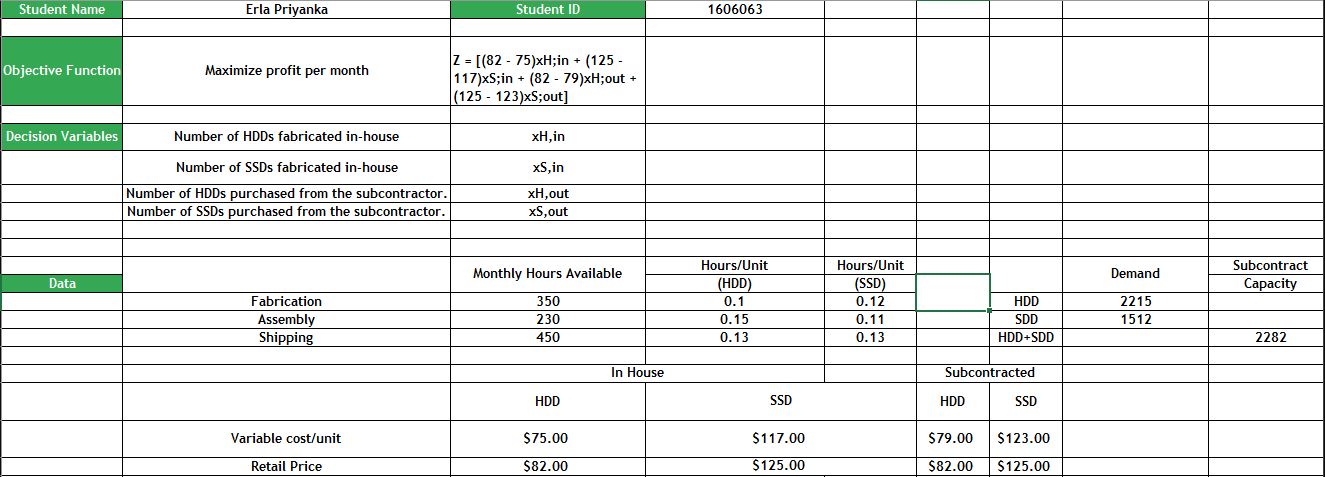
\includegraphics[width=\textwidth]{Q2.PNG} 
\end{center} 



\end{document}
